%----------------------------------------------------------------------------
\chapter{Technológiai ismertető}
\label{chap:techPrim}
%----------------------------------------------------------------------------

\section{Programozási paradigmák fejlődése}

Napjaink nagyméretű, sokszor többmilliónyi kódsorból álló szoftverrendszereinek kifejlesztése elképzelhetetlen lenne előzetes rendszertervezés nélkül.
A különféle tervezésmódszertanok nyomot hagytak a szoftverek tervezési módszerein is.
Egyik híres módszertan a Barry Boehm által 1986-ban publikált Spirál modell \cite{Boehm:1986:SMS:12944.12948}, melyben a fejlesztés szokásos fázisai -- követelmény specifikáció, feladatelemzés, architekturális tervezés, algoritmikus tervezés, implementálás, tesztelés -- mellett megjelenik az élet folytonosságát kifejező, magasabb szinten való ismétlődése a fejlesztési lépéseknek.
A különböző szoftverfejlesztési paradigmák -- moduláris, strukturális, objektum orientált, komponens alapú, aspektus orientált, generikus (template alapú), evolúciós, intencionális, multiparadigmás -- nélkül a nagyméretű, korszerű programrendszerek előállítása lehetetlen volna.
A modern szoftverfejlesztést támogató -- \gls{CASE}, computer-aided software engineering -- eszközök egyik ismert tagja az említett tervezési folyamat első lépéseit támogató Unified Modeling Language (\gls{UML}).
A fejlett szoftverparadigmák mindegyike kiemelten kezeli a modellezés különböző szintjeinek gépi támogatását.
Ismert tény, hogy az adott programnyelven történő implementálás időigényének nagyságrendjébe esik a tesztelés és az előzetes rendszertervezés időigénye is, így ezek automatizálásának szándéka érthető.

%----------------------------------------------------------------------------

\section{A modellezés előnyei}

A \emph{modell} definíciója szerint egy rendszer, elmélet, vagy jelenség leírása, mely rendelkezik annak ismert, vagy kikövetkeztetett tulajdonságaival és a jellemzői további vizsgálatára használható \cite{dict:Model}. 
A szoftverrendszerek tervezésénél többféle modellt alkalmaznak:
\begin{itemize}
	\item adatszerkezeti modell (objektummodell, osztályhierarchia, öröklődés, stb.)
	\item funkcionális modell (adatforrások, -tárolók, -nyelők, -folyamok)
	\item dinamikus modell (állapotok, események, kommunikáció) \cite{Kondorosi07}.
\end{itemize}
Az ezen modelleken alapuló nézetek és diagramok -- osztályhierarchia, külső felhasználók, objektumok együttműködése, tevékenységek, események időbelisége, objektumok állapota, rendelkezésre álló szoftver- és hardver erőforrások -- nélkül a tervezés nagy rendszerek esetében áttekinthetetlen, a rendszer implementálás előtti tesztelése, viselkedésének elemzése, idő- és költségbecslések elvégzése kivitelezhetetlen.
A modellezés fejlődése a szoftverfejlesztésben a 2000-es évekre elvezetett a \emph{modell-vezérelt paradigmák} -- model-driven software development (\gls{MDSD}), model-driven engineering (\gls{MDE}), model-driven architecture (\gls{MDA}) -- és eszközrendszerek kifejlődéséhez \cite{OMG:MDA:FAQ,Schmidt:MDE:10.1109/MC.2006.58,MDSD:TEM06}.

%----------------------------------------------------------------------------

\section{Platformfüggetlen szoftvermodellezés}

Az \gls{OMG} által fejlesztett \gls{MDA} metodológia a szoftverrendszer funkcionalitását platformfüggetlen modell (\gls{PIM}, platform-independent model) alkalmazásával, megfelelő doménspecifikus leírónyelv (\gls{DSL}, domain-specific language) segítségével definiálja.
A modell-vezérelt architektúrához (\gls{MDA}) kapcsolódik többek között a jól ismert \gls{UML} rendszermodellező nyelv és az \gls{XMI} (XML Metadata Interchange) metaadatok XML-alapú cseréjét biztosító szabvány is \cite{OMG:MDA:Spec}. 
Az \gls{MDA} által felhasznált eszközök az alábbi kategóriákba sorolhatóak:
\begin{itemize}
	\item \emph{szerkesztő eszközök} (creation tools) modellek létrehozására, szerkesztésére
	\item \emph{elemző eszközök} (analysis tools) a modellek teljességének, konzisztens szerkezetének, hibamentességének ellenőrzésére, szoftvermetrikák számítására
	\item \emph{transzformációs eszközök} (transformation tools) meglévő modellek más modellekbe alakításhoz, vagy programnyelvekre fordításhoz, dokumentáláshoz
	\item \emph{kompozíciós eszközök} (composition tools) több forrásmodell egy modellé egyesítéséhez
	\item \emph{tesztelő eszközök} (test tools) a modellek teszteléséhez
	\item \emph{szimulációs eszközök} (simulation tools) a modell által leírt rendszer működésének szimulálásához
	\item \emph{metaadat menedzselő eszközök} (metadata management tools) különböző modellek közti általános kapcsolatok és metaadatok -- pl. létrehozó, létrehozási idő, stb. -- kezelésére
	\item \emph{visszafejtő eszközök} (reverse engineering tools) idejétmúlt modellek vagy más információhordozók teljes értékű modellekké alakítására.
\end{itemize}

A szakdolgozatom keretében kifejlesztendő komponensek modell-lekérdezések -- melyekre szintén tekinthetünk modellként -- analízisére lesznek alkalmasak, emiatt az elemző eszközök közé tartoznak.

Egy konkrét szoftverfejlesztési platform megadása után megtörténik a platformfüggetlen modell transzformációja az adott, konkrét platformon működő modellre (\gls{PSM}, platform-specific model).
Ezt a transzformációt leírhatjuk többek közt egy modelltranszformációs nyelv (\gls{MTL}) segítségével, amilyen pl. a VIATRA2 Textual Command Language \cite{Balogh:2006:AMT:1141277.1141575}.

%----------------------------------------------------------------------------

\section{Platform-specifikus szoftvermodellezés}

Míg az \gls{MDA} nyújtja a platformfüggetlenséggel az általános modellezés magas szintjét és az ebből eredő átjárhatóságot a platformok között, addig a konkrét alkalmazások létrehozásához az \gls{MDA}-ban készült platformfüggetlen modellt (\gls{PIM}) le kell fordítani egy adott szoftverplatformra.
Ennek a fordításnak az eredményeként a szoftvermodell valamilyen doménspecifikus környezeten áll elő, mely jelenthet pl. egy Java nyelvi környezetet is.

A specializálódás előnyökkel és hátrányokkal is jár.
Az előnyök között említhetjük a doménspecifikus szoftvertechnológia nagyobb hatékonyságát, adott területen akár félkész megoldást nyújtó jellegét, a modellezett feladat természetéhez való jobb illeszkedést, pl. a Prolog nyelv -- a futtatókörnyezetében -- beépítetten tartalmazz egy következtető automatát, ami szakértőrendszer alkalmazások írásakor már fél megoldást ad.
Ugyanakkor a specializálódásból származnak hátrányok is: az átjárhatóság, magasabb szintű absztrakciók elvesztése, speciális programozási ismeretek iránti igény, a hordozhatóság csökkenése.
Egy közbenső szintet jelent a doménspecifikus modellezés nyelveinek (\gls{DSML}, domain-specific modeling language) alkalmazása, melyek a \gls{DSM} szoftverfejlesztési metodológia eszközeként az \gls{MDA}-tól specifikusabb, de az általános célú programozási nyelvektől (pl. \CPP, Java, \CSharp) általánosabb reprezentációs szintet képviselnek \cite{Kelly2008}.
Ezen a szinten, illetve \gls{DSML} nyelven leírva a programozási feladatot, már alkalmazhatunk automatikus kódgenerálást is, amely valamely általános programnyelvre fordítja a formális modellünket.
A \gls{DSML} nyelven való feladatleírás könnyebbsége és kisebb részletesség iránti igénye az ily módon végzett szoftverfejlesztés hatékonyságában is megmutatkozik, mely összemérhető a \gls{CASE} eszközök, illetve az \gls{UML} hatékonyságával és absztrakciós szintjével, de azoktól korszerűbb, és azoktól szélesebb körben használható.

A \gls{DSM} környezetek a magas szintű leírónyelven és az abból általános programnyelvű kódot generáló fordítón kívül általában további általánosan használt alapszolgáltatásokat is nyújtanak.
A következőkben egy ilyen környezetet, az Eclipse Modeling Framework-öt (\gls{EMF}) mutatom be, mivel az EMF-IncQuery keretrendszer és ezáltal a feladatom jelentős része is erre épül.
Az \gls{EMF} az Eclipse nyílt forráskódú, platformfüggetlen magas szintű szoftverfejlesztési környezet általános modellező keretrendszere.

%----------------------------------------------------------------------------

\section{Az Eclipse integrált szoftverfejlesztő keretrendszer}

Az elsősorban Java nyelven íródott Eclipse integrált fejlesztő környezet (Integrated Development Environment, IDE) egy elsődlegesen Java szoftverek fejlesztésére alkalmas eszköz (lásd \ref{fig:EclipseIDE}. ábrán), ám az alap munkakörnyezeten kívül -- a meglehetősen gazdag beépülő-modul készletének köszönhetően -- számtalan további programnyelven teszi lehetővé a fejlesztést.
%
\begin{figure}[hbt]
\centering
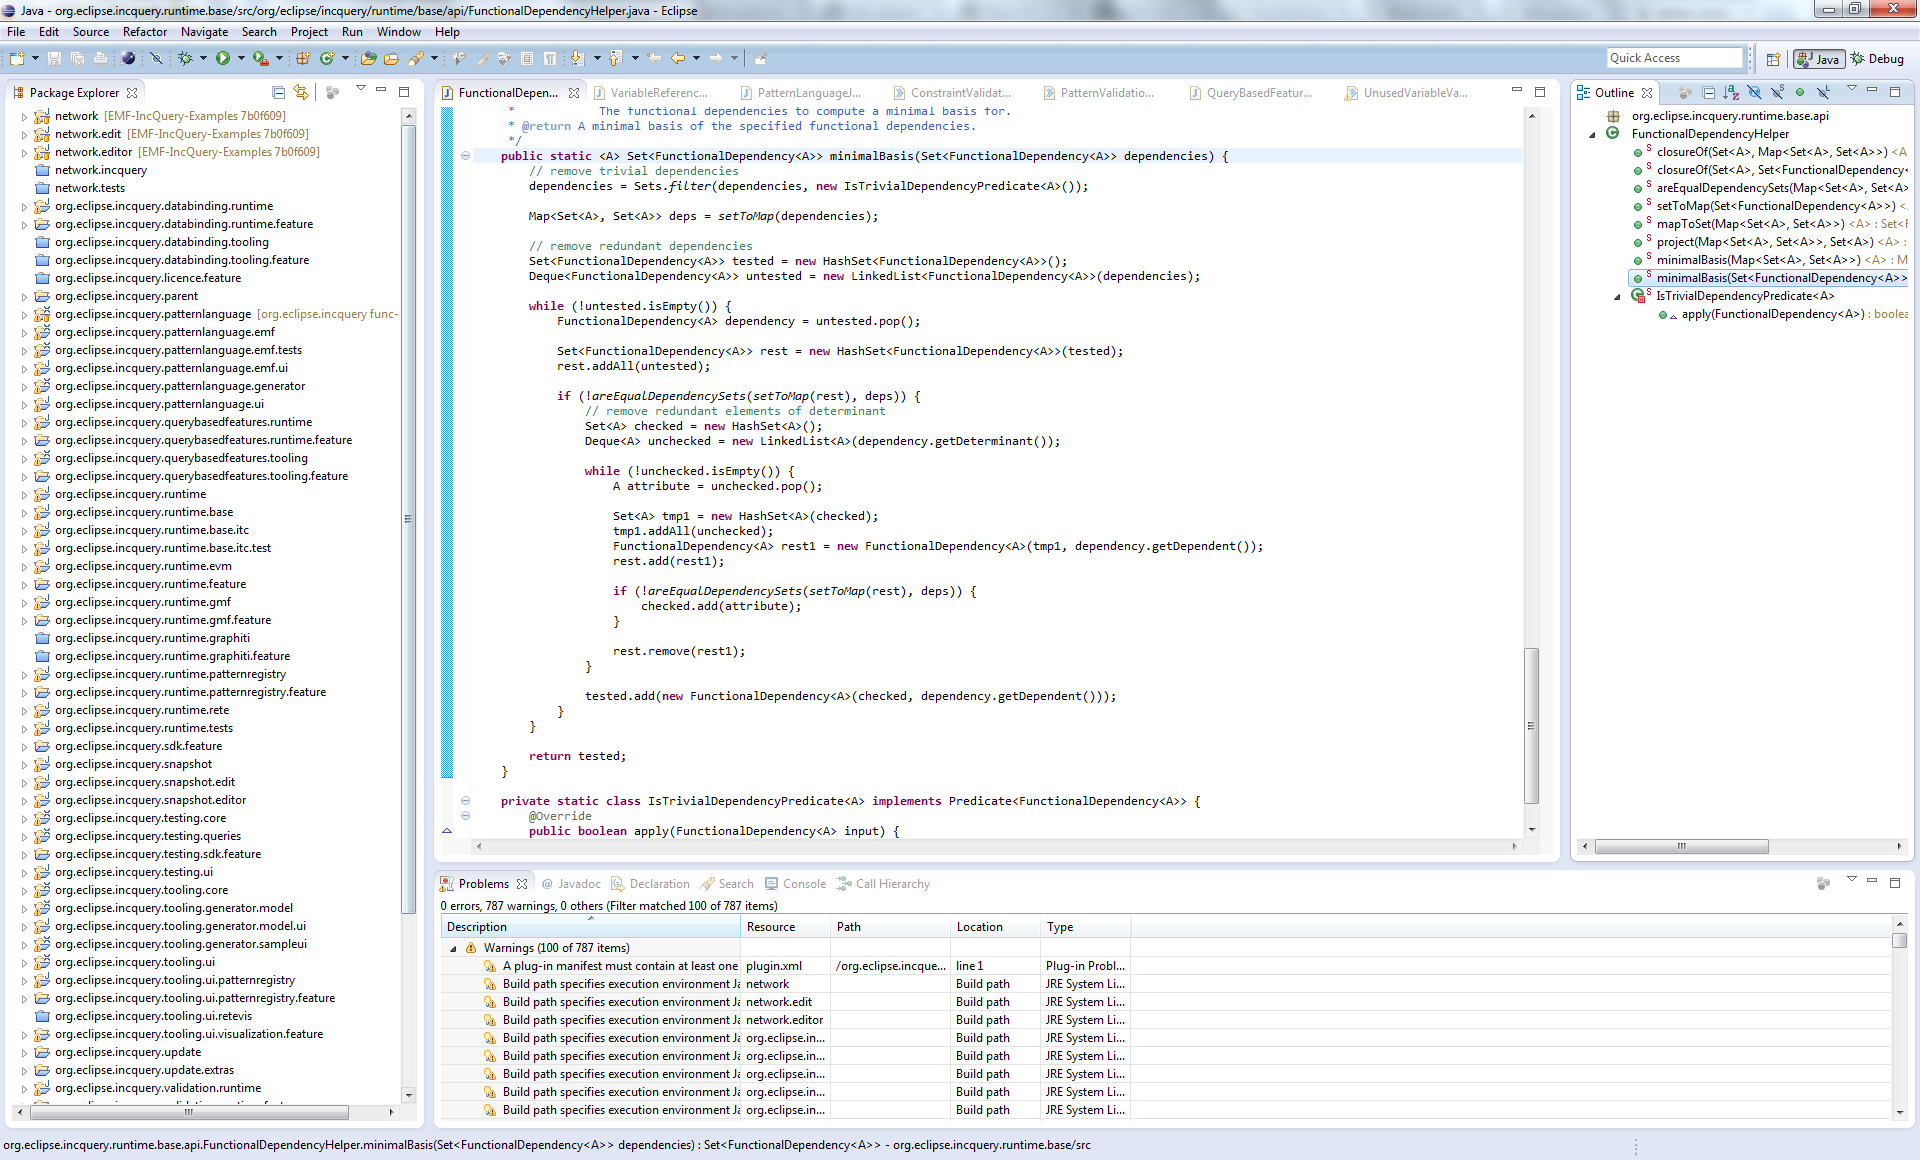
\includegraphics[width=\textwidth]{figures/eclipse-ide.png}
\caption{Eclipse fejlesztőkörnyezet Windows 7 operációs rendszeren}
\label{fig:EclipseIDE}
\end{figure}
%
Ilyen nyelvek többek között az Ada, C/\CPP, Clojure, COBOL, Erlang, FORTRAN, Haskell, JavaScript, Perl, PHP, Python, R, Ruby, Scala, Scheme.
Az Eclipse céljaiban hasonlít a Microsoft Visual Studio, vagy az Embarcadero Rapid Application Development (RAD) Studio integrált többnyelvű szoftverfejlesztő környezetére.
Platformfüggetlenségét Linux, Mac OS X, Solaris és Windows operációs rendszereken való futtathatósága jelenti.
A nyílt forráskódú környezet és hozzá kapcsolódó egyéb projektek rendszeres továbbfejlesztésről és új összetevők hozzáadásáról a lelkes és nyílt fejlesztői közösség  gondoskodik az Eclipse Foundation irányítása mellett.
%A legutóbbi 4.3 verzió a Kepler nevet viseli és 2013. június 26-án jelent meg, de már folyik a legújabb, Luna projekt is \cite{wiki:EclipseIDE}. 

Az integrált szoftverelemek felölelik a szoftverfejlesztés majd minden fázisát.
A fejlesztést szolgáló projektekről az Eclipse-közösség főoldaláról elérhető Projects (\url{http://projects.eclipse.org/}) lapon tájékozódhatunk.
A különböző fejlesztési fázisában lévő 235 fő- és alprojekt mutatja a kezdeményezés nagyságát.
A fő projektek között megtaláljuk a
\begin{itemize}
    \item Business Intelligence and Reporting Tools (BIRT)
    \item Data Tools Platform
    \item Eclipse Project
    \item Eclipse Modeling Project
    \item Mylyn
    \item RT
    \item SOA Platform Project
    \item Technology Project 
    \item Tools Project
    \item Eclipse Web Tools Platform Project
\end{itemize}
főágakat, melyek közül számunkra a dolgozat témája miatt legfontosabb az Eclipse Modeling Project főág a benne található Eclipse Modeling Framework (\gls{EMF}), \mbox{Xtext} és \mbox{VIATRA2} alprojektek miatt, mivel ezek kapcsolódnak legszorosabban az EMF-IncQuery-hez, de az Eclipse Project főág is említésre méltó.

Az Eclipse Project célja egy nyílt forráskódú, robusztus, általános célú, ipari színvonalú platform kidolgozása, mely magas szinten integrált komponensekkel segíti az alkalmazások fejlesztését.
Ennek eléréséhez nyújt támogatást a Plug-in Development Environment (PDE) Eclipse beépülő modulok és egyéb Eclipse platformra épülő eszközök kifejlesztésének elősegítésével.
Az alprojekt széleskörű \gls{OSGi} eszközkészletet is szolgáltat, mely ideális környezetté teszi komponens programozáshoz is a beépülő-modul fejlesztésen túl \cite{EclipseOrgPDE}.

Az EMF-IncQuery keretrendszernek részei olyan komponensek, melyek a PDE-et felhasználva beépülnek az Eclipse fejlesztői környezetbe, ahol varázslókkal és fejlesztési idejű ellenőrzésekkel támogatják lekérdezések definiálását az EMF-IncQuery szöveges tárgynyelvén vagy akár grafikus formában \cite{Gyorok13}, továbbá lehetővé teszik az elkészült lekérdezések interaktív futtatását \gls{EMF} példánymodelleken.

%----------------------------------------------------------------------------

\section{Az Eclipse Modeling Framework}

Az Eclipse Modeling Framework (\gls{EMF}) adatszerkezetek, domének modellezésére szolgáló keretrendszer, mely modell-vezérelt szoftverfejlesztést tesz lehetővé, vagyis képes a modellezett adatszerkezetek Java kódjának generálására is \cite{VogelEMF}.
Ily módon könnyen áttekinthető vizuális támogatással és grafikus szerkesztővel hozhatunk létre robusztus, nagyméretű adatrendszer modelleket, melyekből a közvetlen kódgenerálás is megoldott.
Az \gls{EMF} előnyei között említendő a csoportmunka támogatása is.
Az adatszerkezetek modellezésére vonatkozó ajánlás azok elkülönítése a programkódtól, ily módon csak adattagokat tartalmazó osztályok definiálása.

Az \gls{EMF} megkülönbözteti az adatmodell modelljét, azaz az adatmodell szerkezetét leíró meta-modellt az aktuális modelltől, mely a meta-modell egy példányaként fogható fel. 
Az \gls{EMF} modellező széles elterjedtségét magyarázza a magas szintű modellezés kivitelezésének könnyű volta, az erős integráltsága az Eclipse alá, továbbá az automatikus kódgenerálás.
Számtalan alkalmazása közül megemlítendő több Eclipse projektben való felhasználása.

A továbbiakban mélyebben elemzem az EMF szerkezetét és lehetőségeit az \url{http://www.eclipse.org/modeling/emf/docs/} weboldalon található áttekintő cikkek \cite{Steinberg:2009:EEM:1197540,VogelEMF} feldolgozása révén.

Meta-modellből kettő található az EMF-ben:
\begin{itemize}
	\item Ecore meta-modell és 
	\item Genmodel meta-modell.
\end{itemize}
Az Ecore meta-modell a definiált osztályokról tartalmaz információt, míg a Genmodel a Java kód generálásához tartalmaz járulékos adatokat, mint pl. fájlnevet és elérési utat, valamint a kódgenerálást vezérlő paramétert.
Az Ecore meta-modell különféle elemek definiálását teszi lehetővé:
\begin{itemize}
	\item \texttt{EClass}: attribútumokat és/vagy hivatkozásokat tartalmazó osztály
	\item \texttt{EAttribute}: névvel és típussal rendelkező attribútum
	\item \texttt{EReference}: két osztály közötti kapcsolat egyik végét reprezentálja; egy flag-gel jelzi, ha tartalmazást reprezentál
	\item \texttt{EDataType}: adattípus, pl. \texttt{int}, \texttt{float}, \texttt{java.util.Date}.
\end{itemize}
%
Az Ecore meta-modell felépítését a \ref{fig:EcoreStruct}. ábra mutatja.
%
\begin{figure}[htb]
\centering
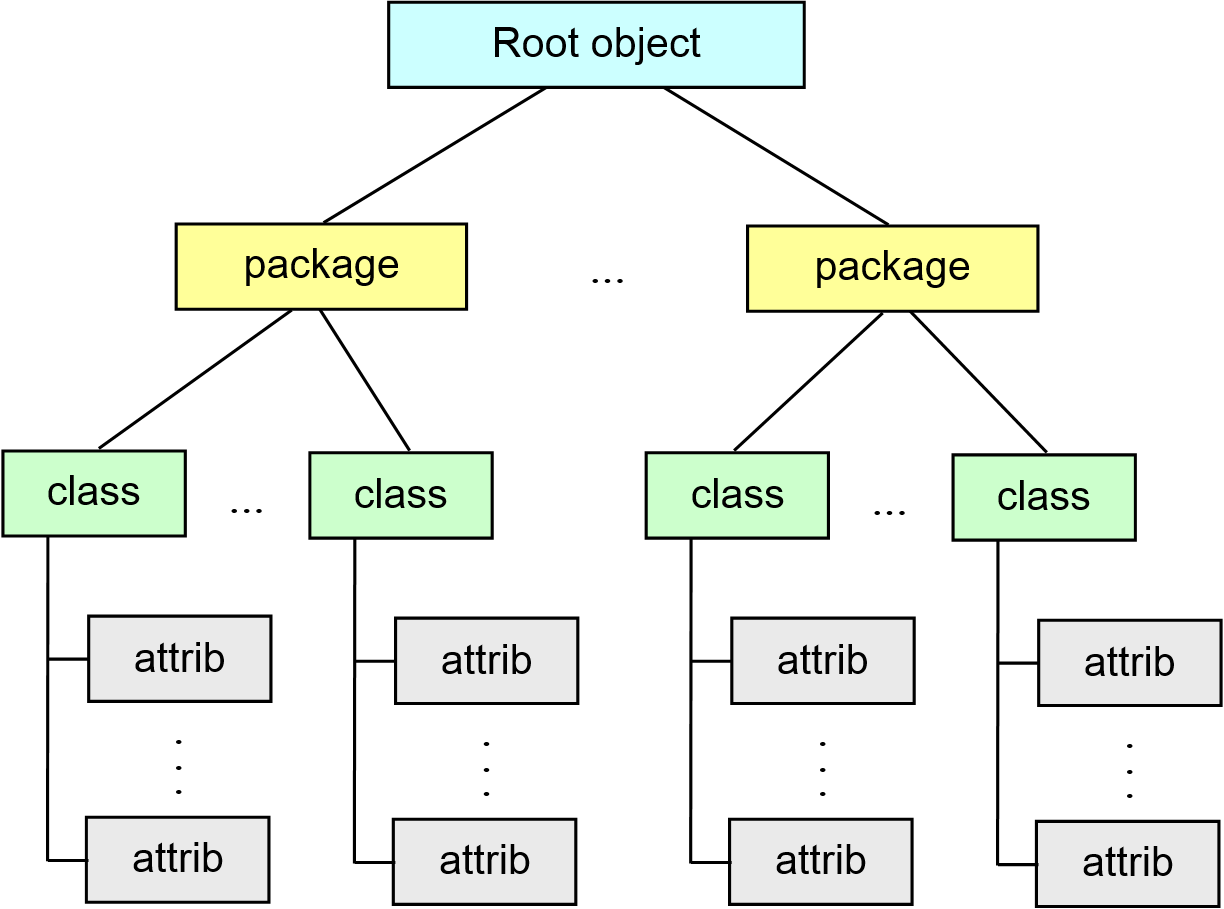
\includegraphics[width=0.8\textwidth]{figures/ecore-metamodel-struct.png}
\caption{Ecore meta-modell szerkezete}
\label{fig:EcoreStruct}
\end{figure}
%
Az Ecore meta-modell fő elemei a \ref{fig:EcoreStruct}. ábra kontextusába helyezve a következők \cite{EMFFundamentals}: 
A gyökér objektum egy EObject elem, ebbe tartoznak az EPackage csomagok, melyek egyszerre kezelendő osztályokból (EClass és EDataType) épülnek fel.
A class szinten EClass elemek reprezentálják a modellezett osztályokat, melyek a nevükből és EAttribute és/vagy EReference elemekből állnak.
Az attribútumoknak neve és típusa is van, míg a referenciák egy bináris kapcsolat egyik irányát modellezik, van nevük és megadják a hivatkozott osztály típusát és a tartalmazásjelző flag-et.
Az adattípust az EDataType elem adhatja meg.  

Az alkalmazások konkrét adatmodelljei az Ecore meta-modell egyedei.
A \ref{fig:DataModelWithXMI}. ábra mutat egy konkrét példát egy alkalmazás adatmodelljére.
%
\begin{figure}[htb]
\centering
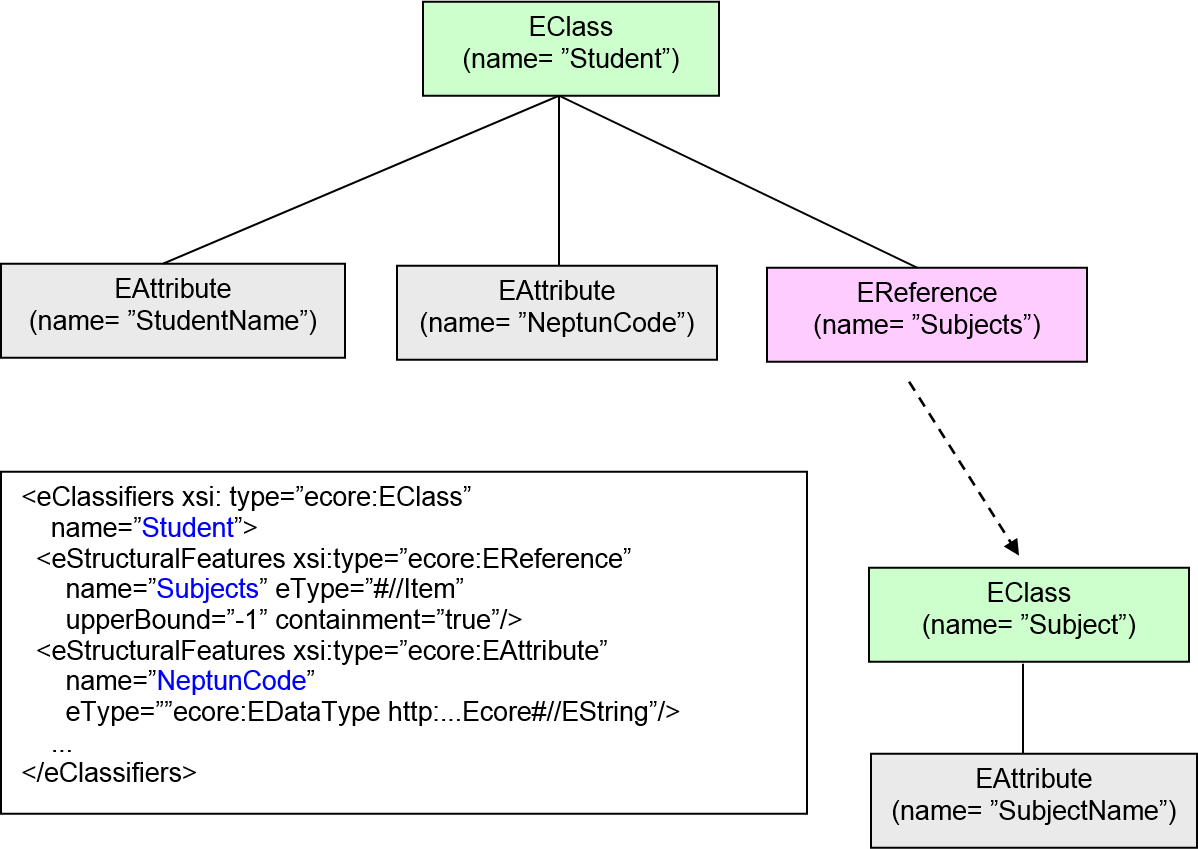
\includegraphics[width=\textwidth]{figures/datamodel-example-with-xmi-desc.png}
\caption{Alkalmazás adatmodell példa, XMI formátumú megadással}
\label{fig:DataModelWithXMI}
\end{figure}
%
Az EMF modell lényegében az UML osztálydiagram nézetének egy részhalmaza \cite{EMFFundamentals}.
Az EMF modellek az alábbi módokon is megadhatók:
\begin{enumerate}
	\item Java Interfaces
	\item UML Class Diagram
	\item XML Schema
\end{enumerate}
A modellimport és a kódgenerálás lehetőségeit a \ref{fig:ModelImportAndCodegen}. ábrán láthatjuk \cite{EMFFundamentals}.
%
\begin{figure}[!b]
\centering
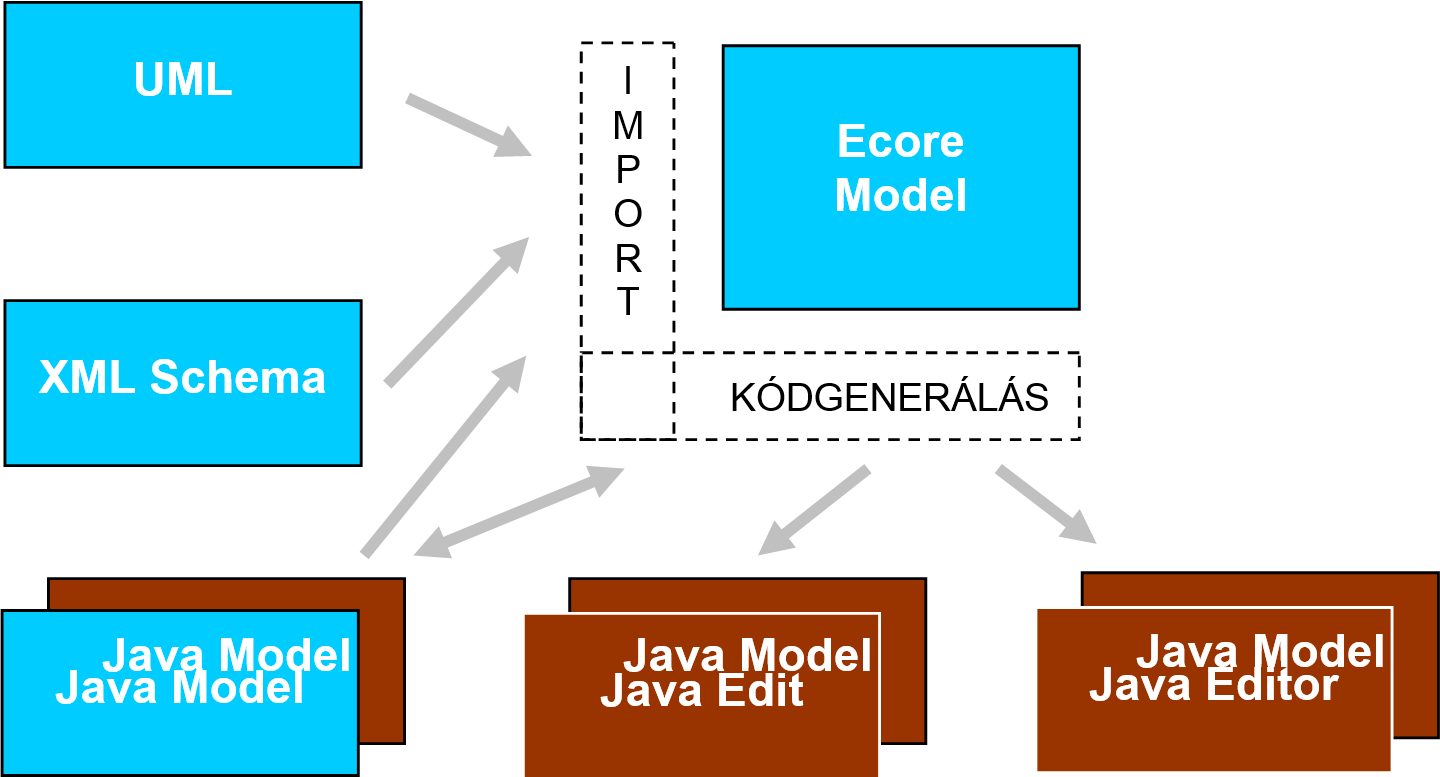
\includegraphics[width=\textwidth]{figures/model-import-and-codegen.png}
\caption{Modell import és kódgenerálás}
\label{fig:ModelImportAndCodegen}
\end{figure}
%
A kódgenerálás oda-vissza működik, Ecore modell generálható annotált Java interfészekből \cite{MasteringEMF}.
A generált kód tartalmazza az interfészt és az osztály implementációt, pl. a \ref{fig:DataModelWithXMI}. ábra szerinti modell esetén a következő formában:
%
\begin{lstlisting}
public interface Student extends EObject
{
    String getStudentName();
    void setStudentName(String value);
    String getNeptunCode();
    void setNeptunCode(String value);
    EList<Subject> getSubjects();
}
\end{lstlisting}
\begin{lstlisting}
public class StudentImpl extends EObjectImpl
    implements Student
{
    ...
}
\end{lstlisting}
A programkód tartalmazza a getter/setter elérőfüggvényeket az attribútumokhoz és a referenciákhoz.

Az EMF meta-modell létrehozását az \ref{fig:EcoreDiagramEditor}. ábra szerinti grafikus szerkesztő segíti.
%
\begin{figure}[htb]
\centering
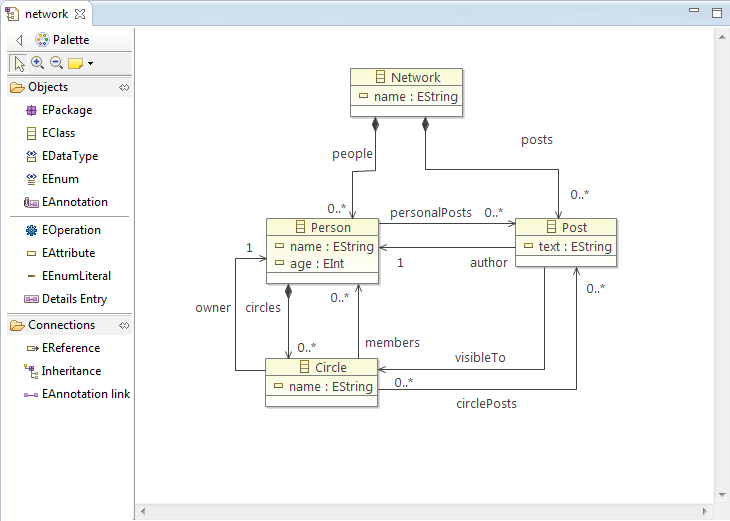
\includegraphics[width=\textwidth]{figures/ecore-diag-editor.png}
\caption{Ecore grafikus modellszerkesztő}
\label{fig:EcoreDiagramEditor}
\end{figure}
%
Egy példát egy adatszerkezetre \cite{VogelEMF} alapján a \ref{fig:EcoreMetaModelExample}. ábra mutat.
%
\begin{figure}[htb]
\centering
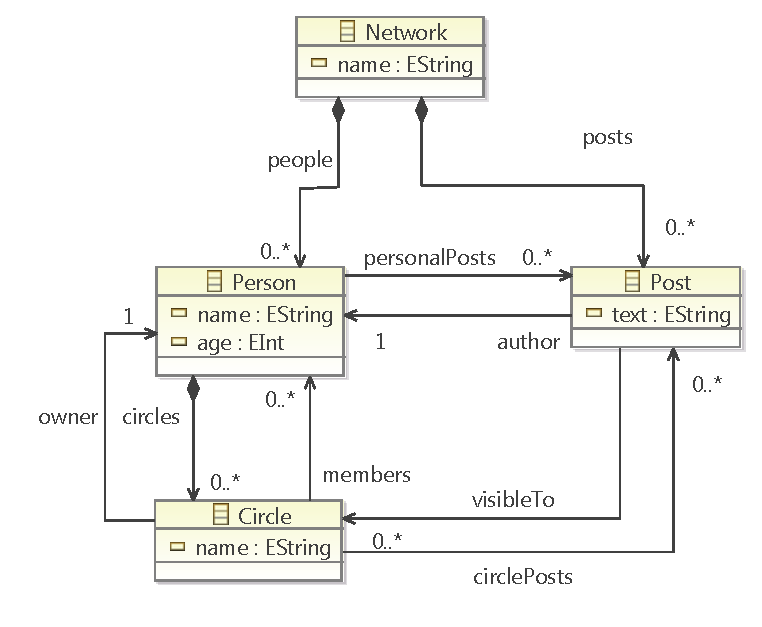
\includegraphics[width=\textwidth]{figures/ecore-network-metamodel-diag.pdf}
\caption{Példa Ecore meta-modellre (Network modell)}
\label{fig:EcoreMetaModelExample}
\end{figure}

A dolgozatban kulcsszerepet játszó Eclipse Modeling Framework (\gls{EMF}) bemutatásának összefoglalásaként a következőket emelhetjük ki \cite{EMFFundamentals}:
Az \gls{EMF} a legkézenfekvőbb modellező eszköz a Java környezet számára.
Az alkalmazás belső modelljére épít, nem szükséges más magas szintű modellező eszköz.
A modellezést és a programozást keverten is képes kezelni növelve ezáltal mindkettő hatásfokát.
A szoftverfejlesztés termelékenységét növeli és megkönnyíti az integrációt.
Mindezek alapján az Eclipse modell alapú fejlesztésének és adatintegrációjának az alapja. 

A feladatkiírás szerint az \gls{EMF}-re épülő, a Budapesti Műszaki Egyetem Méréstechnika és Információs Rendszerek Tanszékének Hibatűrő Rendszerek Kutatócsoportja által kidolgozott, modell-lekérdezések végrehajtására alkalmas EMF-IncQuery keretrendszerben kell vizsgálatokat végeznem, ezért a következőkben ezt a keretrendszert ismertetem.

%----------------------------------------------------------------------------

\section{EMF-IncQuery}\label{sect:IncQuery}

A szekció célja bemutatni az EMF-IncQuery és a lekérdezőnyelv felépítését, használatát, továbbá, a feladatkiírás első pontjának megfelelően, a modell-lekérdezések fogalmát az EMF-IncQuery keretrendszeren keresztül.

A keretrendszer főbb tulajdonságait röviden a \cite{EMFIncQuery} foglalja össze:
Az EMF-IncQuery \gls{EMF} modelleken végzendő deklaratív lekérdezések definiálására és végrehajtására alkalmas keretrendszer.
Fontos jellemzője, hogy a definiált lekérdezéseket kézi programírás nélkül, hatékonyan hajthatjuk végre.
A lekérdezőnyelv a gráfmintázatok módszerét alkalmazza, amely tömör és egyszerű eljárás komplex szerkezetű modell-lekérdezések megadására.
A kiemelkedő futási teljesítményt azáltal nyújtja, hogy inkrementális gráfminta illesztési technikákat alkalmaz.
Ennek köszönhetően a keresés még milliós nagyságrendű elemszám mellett is gyors.
Emellett az \gls{EMF} pár hiányosságát is orvosolja, mint például az osztályok egyedinek gyors és hatékony felsorolása helyre való tekintet nélkül, egyszerű fordított navigáció bármilyen referencia mentén, és objektumok megkeresése attribútum érték alapján.
Az újabb verzió képes származtatott tulajdonságok -- virtuális attribútumok és referenciák -- kiértékelésére is.

\subsection{Felépítés}

Az EMF-IncQuery felépítését a \ref{fig:EMFIncQueryStructure}. ábra mutatja \cite{Bergmann-TOOLS-2012}.
%
\begin{figure}[htb]
\centering
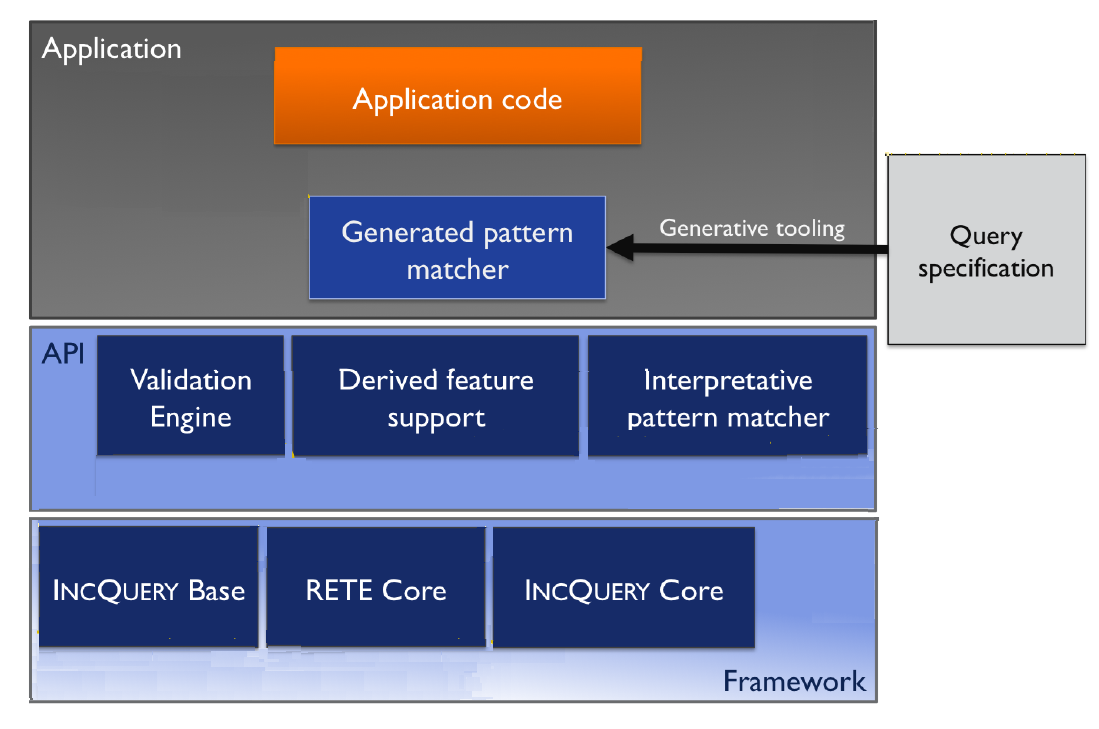
\includegraphics[width=\textwidth]{figures/emf-incquery-structure.png}
\caption{Az EMF-IncQuery felépítése}
\label{fig:EMFIncQueryStructure}
\end{figure}
%
A megadott lekérdezésen (Query specification) alapulva mintaellenőrző pluginok generálódnak (Generated pattern matcher), melyek könnyen integrálhatók egy meglévő Eclipse-alapú alkalmazásba (Application, Application code).
A lekérdezés megadását Xtext 2-alapú szerkesztő támogatja, amely fejlett szintaxis kiemeléssel, kódkiegészítéssel és formula ellenőrzéssel rendelkezik.
Ezek a pluginok az EMF-IncQuery API-n keresztül elérik a rendszer belső funkcionalitását.
Az API-ban a Validation Engine, validáló motor körbeveszi az EMF Validációs szolgáltatást  (Validation Service), hogy EMF-IncQuery-alapú online jól formáltság ellenőrzést végezve a validátorai révén szabványos Eclipse hiba markereket nyújtson.
Másodsorban az interpretáló mintaellenőrző (Interpretative pattern matcher) a Java kódból származó közvetlen lekérdezések számára elérési pontot nyújt azok gyors végrehajtásához.
Az API nyújtja továbbá a származtatott sajátosságok támogatását (Derived feature support).
A keretrendszerben a Base komponens gyakran használt alacsony szintű inkrementális lekérdezéseket nyújt, mint pl. a már említett egyed felsorolások, és fordított irányú navigálás egyirányú hivatkozásokon.
A lekérdezések inkrementális kiértékelését és életciklus kezelését a RETE motor szolgáltatja (RETE Core).
Az IncQuery Core adja az EMF-IncQuery keretrendszer magját.
A rendszer jellemzőinek mélyebb megértéséhez és az általa nyújtott szolgáltatások feltárásához a \cite{Bergmann-TOOLS-2012} irodalom volt segítségemre.

A gráfmintázatok keresése azzal az előnnyel jár, hogy a gráfminta által reprezentált feltételek vagy korlátozások a modellgráf megtalált, egyező mintázatú részén is teljesülnek.
A gráfminta strukturális, topológiai elvárásokat jelent, megadva az adott típusú élek és csomópontok kereséséhez az információt, továbbá kifejezésekkel az attribútumértékek iránt fogalmaz meg elvárásokat.
Egyes mintarészek/jellemzők kizárhatók az egyezés iránti elvárásból.
A gráfminta keresés ilyen módon nagyon finoman paraméterezett keresések kivitelezésére ad módot.

\subsection{Használat}

Ha egyszerűen csak használni szeretnénk az EMF-IncQuery által nyújtott szolgáltatásokat, akkor nem kell mást tennünk, mint telepíteni az \emph{EMF-IncQuery SDK}-t, illetve a hiányzó függőségeket a már meglévő Eclipse környezetünkbe \cite{EclipseOrgIncQueryInstall}.
Ha azonban újabb komponenseket szeretnénk a keretrendszerhez fejleszteni, akkor a \cite{EclipseOrgIncQueryDevEnv} forrás lesz a segítségünkre.
A fejlesztés megkezdéséhez először le kell tölteni a keretrendszer forráskódját, majd importálni a projekteket a fejlesztői környezetünkbe.
Ezután, az Xtext kódgeneráló munkafolyamatainak (MWE2 szkriptek) végrehajtásával előbb legeneráljuk a lekérdezőnyelv feldolgozásához szükséges kódot, majd javasolt a projekt tisztítása és teljes újrafordítása.
Az eredményt Eclipse Application-ként futtatva, egy olyan Eclipse fejlesztői környezet indul el, amelybe automatikusan betöltődnek az EMF-IncQuery moduljai.

Az így kapott környezetben kipróbálhatjuk az EMF-IncQuery-t: írhatunk lekérdezéseket a tárgynyelven, majd lefuttathatjuk őket példánymodelleken.
Ehhez azonban szükségünk lesz egy modellre.
Ha rendelkezünk már megfelelő EMF modellel, akkor használhatjuk azt, én azonban szeretném röviden bemutatni a modell elkészítésének menetét.

Mint modellezéskor mindig, most is egy domén specifikációjából fogunk kiindulni.
Az általam modellezett domén a karate harcművészetet űzők egy egyszerűsített világa lesz.
Ennek a világnak fő elemei a \emph{karatékák}, a karate harcművészek.
Minden karatékának van neve, és lehet egy meghatározott stílusa.
A karatékák lehetnek \emph{mesterek} vagy \emph{tanítványok}.
A tanítványok egy és csak egy mester alatt tanulhatnak, azonban a mestereknek nem szükségszerű, hogy legyen tanítványuk.
Minden mester a saját \emph{dódzsójában} (edzőterem, klub) oktatja tanítványait, melynek van neve.
Az előző két mondat állításaiból következik, hogy egy tanítvány egyszerre pontosan egy dódzsóban tanulhat.

Ezen leírás alapján elkészíthetjük a domén meta-modelljét az EMF Ecore diagram alapú modellezőjének segítségével.
Ennek mikéntjéről bővebb leírást a \cite{VogelEMF} ad.
Az általam elkészített meta-modellt a \ref{fig:karateMetaModel}. ábra mutatja.
%
\begin{figure}[htb]
\centering
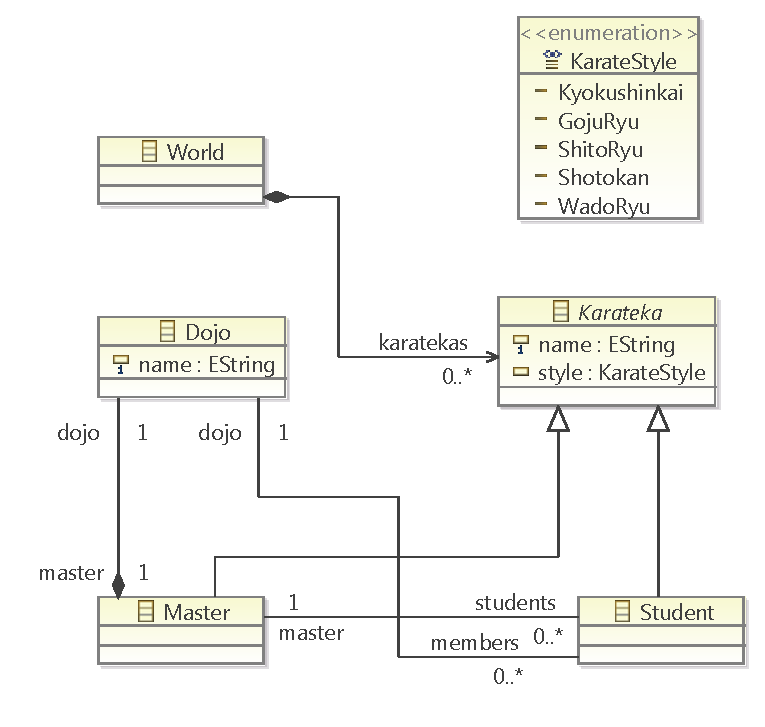
\includegraphics[width=\textwidth]{figures/ecore-karate-metamodel-diag.pdf}
\caption{Karate meta-modell}
\label{fig:karateMetaModel}
\end{figure}
%
Az ábrán látható diagram az UML osztálydiagramok jelölésrendszerét használja.
Jól láthatóak a kapcsolatok a modell főbb elemei közt: a Master és Student osztályok leszármazottjai az absztrakt Karateka osztálynak, megjelennek kétirányú kapcsolatok a Master, Student és Dojo osztályok között.
A KarateStyle a lehetséges karate stílusok felsorolása.
A modell gyökere a World osztály, ez tartalmazza a Karatekakat, akik közül a Master típusúak tartalmazzák a Dojokat.

Az Ecore meta-modell alapján elkészíthetjük a Genmodel meta-modellt, amelyből generálhatjuk modellünk egyedeinek létrehozásához és manipulálásához szükséges Java kódot és az Eclipse-be beépülő szerkesztő komponenseket, melyek segítenek a példánymodellek vizuális konstrukciójában.
A következő lépésben az elkészült komponenseket -- az EMF-IncQuery komponenseivel együtt -- betöltjük az Eclipse környezet egy újabb példányába a már említett módon (futtatás Eclipse Application-ként).
Itt varázsló segítségével létrehozhatjuk a modellünk egy új egyedét, melyet feltölthetünk a szükséges tartalommal.
Én a példánymodellemet a \emph{The Karate Kid} (A karate kölyök) című 1984-es kultuszfilm alapján készítettem el, töltöttem fel adatokkal.
Az elkészült példánymodellt fa formában a \ref{fig:karateInstanceModel}. ábra mutatja.
%
\begin{figure}[htb]
\centering
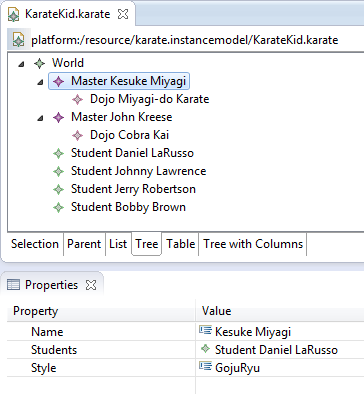
\includegraphics[width=0.70\textwidth]{figures/karate-instance-tree-with-properties.png}
\caption{Karate példánymodell}
\label{fig:karateInstanceModel}
\end{figure}
%

Példánymodellünk kész, jöhet a keresés!
A kereséshez szükségünk lesz egy gráfmintára.
Egy egyszerű, az EMF-IncQuery lekérdezőnyelvén megadott mintát láthatunk a \ref{lst:isStudentOfMiyagiPattern}. kódlistán.
%
\begin{lstlisting}[float,floatplacement=htb,caption=isStudentOfMiyagi gráfminta a tárgynyelven,label=lst:isStudentOfMiyagiPattern]
package karate.incquery

import "http://karate/1.0"

pattern isStudentOfMiyagi(student : Student) = {
    Student.master.name(student, "Kesuke Miyagi");
}
\end{lstlisting}
%
Ha a mintát beregisztráljuk az EMF-IncQuery \emph{Query Explorer} nézetébe és betöltjük mellé a példánymodellünket (\ref{fig:karateInstanceModel}. ábra) is, akkor a lekérdezés automatikusan kiértékelődik, és a \ref{fig:karateQueryResult}. ábrán látható eredményt kapjuk.
%
\begin{figure}[htb]
\centering
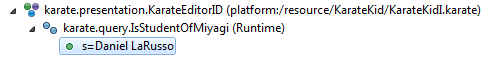
\includegraphics[width=\textwidth]{figures/karate-query-result.png}
\caption{Keresés eredménye}
\label{fig:karateQueryResult}
\end{figure}

\subsection{A lekérdezőnyelv}

A \ref{lst:isStudentOfMiyagiPattern}. kódlistán bemutatott keresési minta az EMF-IncQuery saját, deklaratív gráfminták leírására szolgáló nyelvén (IncQuery Graph Pattern language, IQPL) íródott, mely szintaxisának jelentős részét a VIATRA2 Textual Command Language-ből (VTCL) örökli, szemantikája pedig hasonló a Datalog deklaratív logikai lekérdezőnyelvéhez \cite{Ceri:1989:YAW:627272.627357}.

A nyelv feldolgozását a már említett Xtext keretrendszer végzi, mely programozási és doménspecifikus nyelvek fejlesztéséhez nyúlt alapot: az elemzéstől, a fordításon keresztül, a teljes Eclipse integrációig lefedi a szükséges nyelvi infrastruktúrát.
Az Xtext biztosít olyan eszközöket is, mint a szintaxis kiemelés, a kontextus alapú kiegészítés vagy a validáció.

A nyelv a következő fontosabb elemekből épül fel \cite{EclipseOrgIncQueryLang}:
\begin{description}
\item[Csomag:] a \texttt{package} direktíva -- a Java-hoz hasonlóan -- jelzi, hogy melyik csomag tartalmazza a fájlban lévő mintákat
\item[Importok:] \texttt{import} direktívákkal adhatjuk meg azokat az EMF csomagokat, melyeknek elemeire hivatkozni szeretnénk a lekérdezésekben
\item[Minta:] a \texttt{pattern} kulcsszóval bevezetett minták olyan \emph{predikátumok}, melyeknek lehetnek paramétereik -- melyeknek opcionálisan megadhatjuk a típusát is -- és legalább egy törzsük van; a minta törzsei diszjunktak, vagyis a törzsek logikai VAGY kapcsolatban állnak egymással
\item[Minta-törzs:] a kapcsos zárójelek által határolt minta-törzs legalább egy kényszerből és valahány lokális változóból áll; a törzsben lévő kényszerek logikai ÉS kapcsolatban állnak egymással 
\item[Kényszer:] kényszerek segítségével adhatóak meg a változók tulajdonságai és a közöttük lévő kapcsolatok; egy vagy több változóhivatkozás található bennük
\item[Változó:] értéke megadható, vagy mintaillesztésnél helyettesítődik be; a minta paramétereit \emph{szimbolikus}, a törzsekben találhatóakat pedig \emph{lokális} változóknak nevezzük
\end{description}

A kényszereknek az alábbi fajtái léteznek a nyelvben:
\begin{description}
\item[Összehasonlítás kényszer (\texttt{CompareConstraint}):] ez a kényszer két kifejezés egyenlőségét vagy egyenlőtlenségét határozza meg
\item[Típuskényszer (\texttt{EClassifierConstraint}):] ez a kényszer a paraméterének típusát határozza meg; példa: a \texttt{Student(student);} kifejezés a \texttt{student} változó típusát \textit{Student}-ként határozza meg
\end{description}
\todo{befejezni vagy törölni}